\documentclass{beamer}
\usepackage{../../shared/styles/custom}
\usepackage{../../shared/styles/conventions}
\usepackage{tikz}
\usetikzlibrary{positioning,shapes,arrows}

%\beamerdefaultoverlayspecification{<+->}
% \newcommand{\data}{\mathcal{D}}
% \newcommand\Item[1][]{%
% 	\ifx\relax#1\relax  \item \else \item[#1] \fi
% 	\abovedisplayskip=0pt\abovedisplayshortskip=0pt~\vspace*{-\baselineskip}}

\graphicspath{ {../assets/bias-variance/figures/} }



\title{Bias-Variance and Cross Validation}
\date{\today}
\author{Nipun Batra and teaching staff}
\institute{IIT Gandhinagar}
\begin{document}
\maketitle

\begin{frame}{Table of Contents}
\tableofcontents
\end{frame}

\section{Introduction to Bias-Variance}

\begin{frame}{What is the Bias-Variance Tradeoff?}
\begin{alertbox}{The Central Challenge in Machine Learning}
\textbf{Every ML model faces a fundamental tension:}
\begin{itemize}
\item Make simple assumptions → Miss important patterns (High Bias)
\item Make complex assumptions → Overfit to noise (High Variance)
\end{itemize}
\end{alertbox}

%\vspace{0.3em}
\textbf{Today's Goal:} Understand this tradeoff through intuitive examples, mathematical foundations, and practical techniques.

\begin{keypointsbox}
\textbf{Key Questions We'll Answer:}
\begin{itemize}
\item What exactly are bias and variance?
\item How do they affect model performance?
\item How can we find the optimal balance?
\end{itemize}
\end{keypointsbox}
\end{frame}

\begin{frame}{A Real-World Analogy: Weather Prediction}
\begin{examplebox}{Simple Model: "Tomorrow = Today"}
\textbf{High Bias:} Ignores weather patterns \\
\textbf{Low Variance:} Always makes same type of prediction
\end{examplebox}

\begin{examplebox}{Complex Model: 1000+ Variables}
\textbf{Low Bias:} Can capture complex patterns \\
\textbf{High Variance:} Small errors → wildly different forecasts
\end{examplebox}

\textbf{Goal:} Find the sweet spot between these extremes
\end{frame}

\begin{frame}{A Question!}
	What would be the decision boundary of a decision tree classifier? 
		
	\begin{figure}
		\centering
	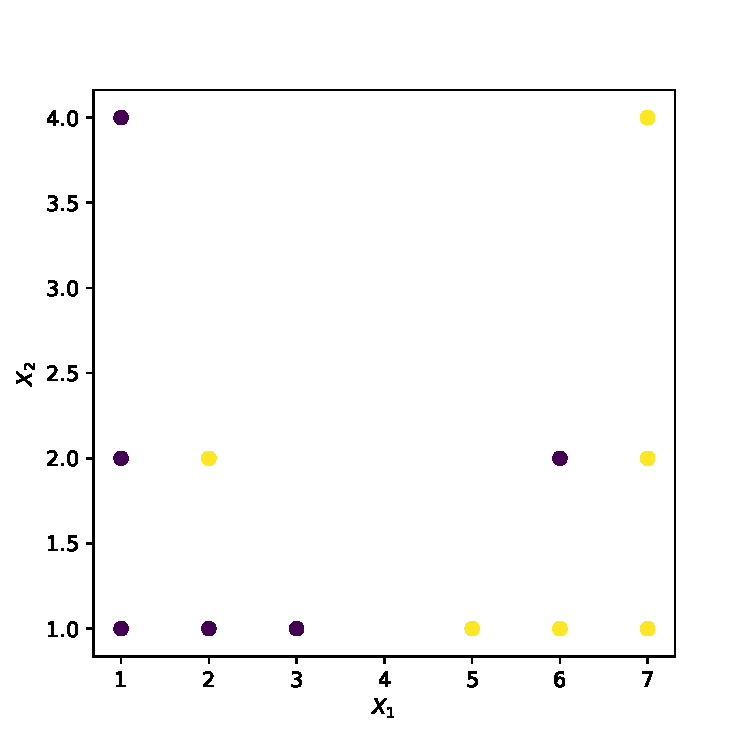
\includegraphics[scale=0.55]{dataset-1}
	\end{figure}


	\end{frame}

	\begin{frame}{Decision Boundary for a tree with depth 1}
	\begin{figure}[h]
	    \centering
	    \begin{minipage}{0.45\textwidth}
	        \centering
	        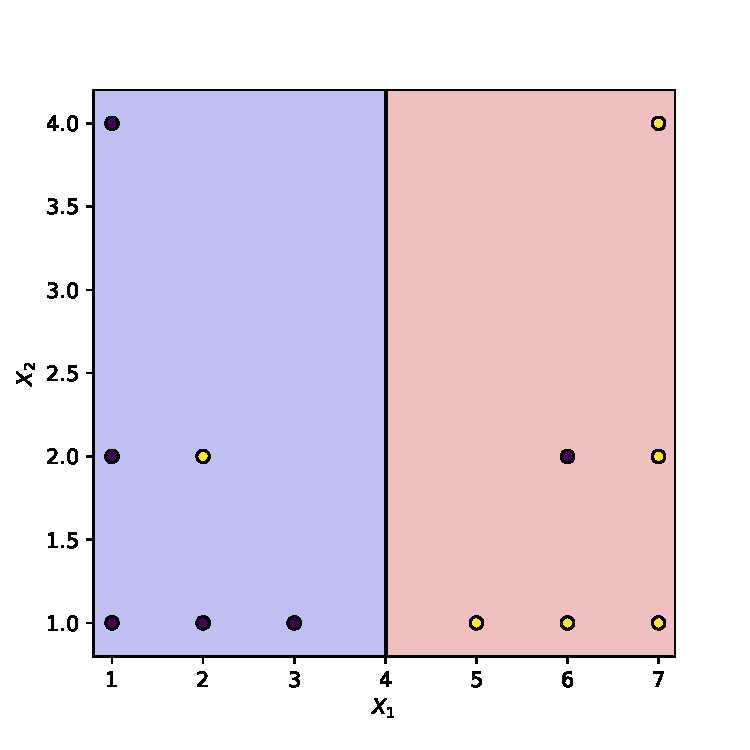
\includegraphics[width=\textwidth]{example-1-depth-1-boundary}
	        \caption{Decision Boundary}
	    \end{minipage}
	    \hfill
	    \begin{minipage}{0.45\textwidth}
	        \centering
	        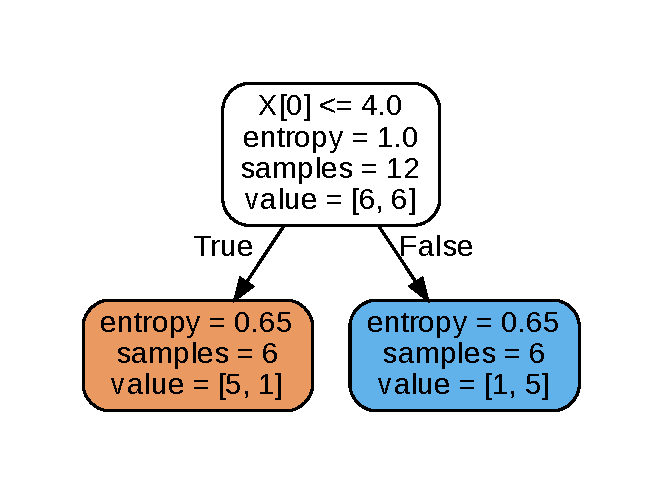
\includegraphics[width=\textwidth]{example-1-depth-1-decision-tree}
	        \caption{Decision Tree}
	    \end{minipage}
	\end{figure}
	\end{frame}
	
	\begin{frame}{Decision Boundary for a tree with no depth limit}
	\begin{figure}[h]
	    \centering
	    \begin{minipage}{0.45\textwidth}
	        \centering
	        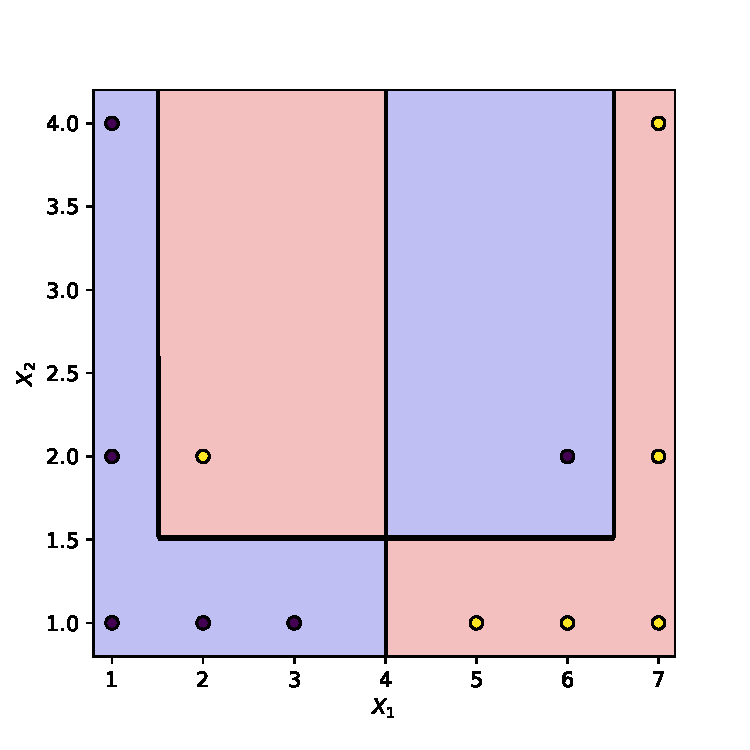
\includegraphics[width=\textwidth]{example-1-nolimit-boundary}
	        \caption{Decision Boundary}
	    \end{minipage}
	    \hfill
	    \begin{minipage}{0.45\textwidth}
	        \centering
	        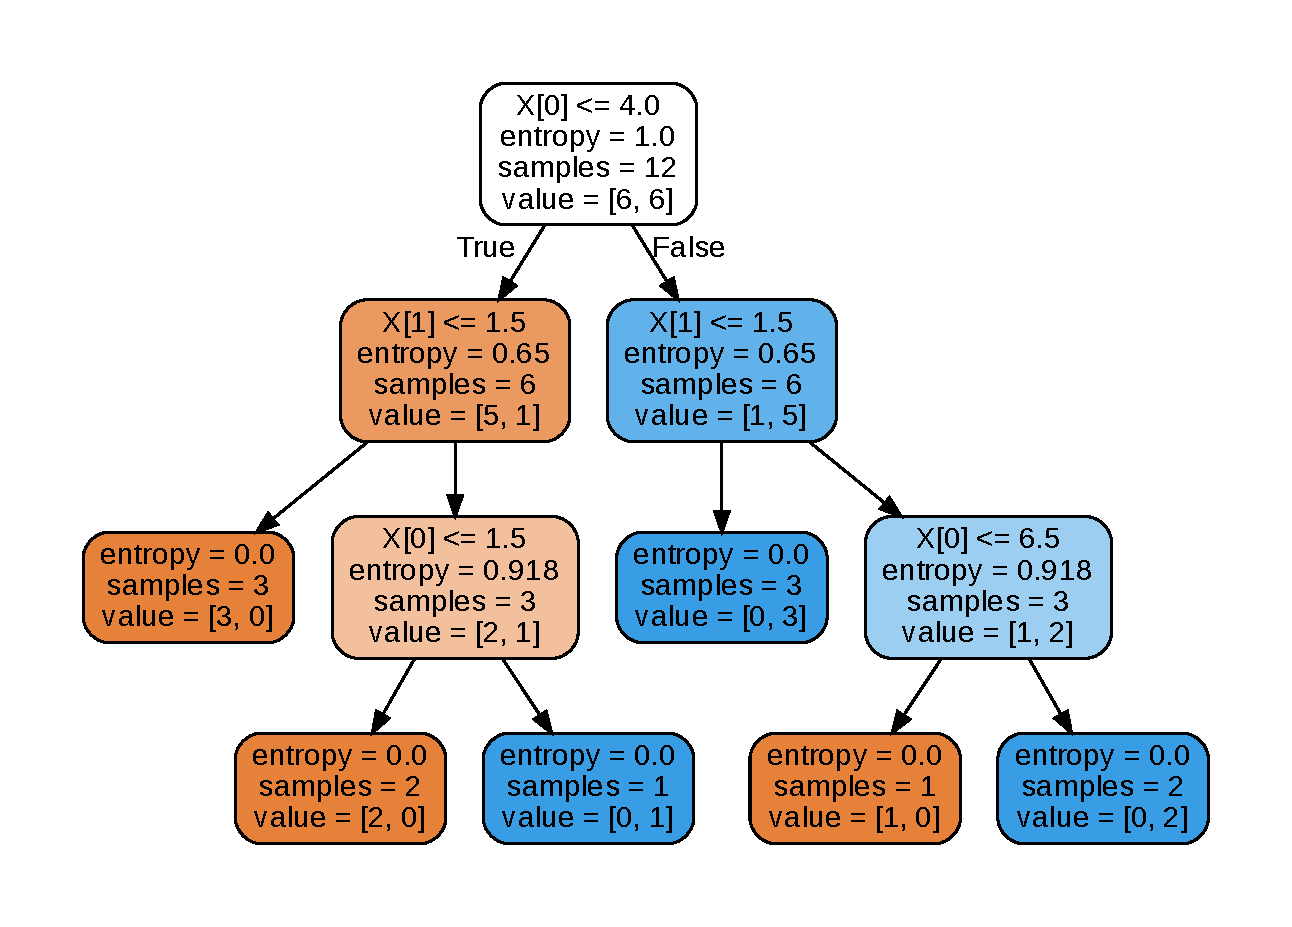
\includegraphics[width=\textwidth]{example-1-nolimit-decision-tree}
	        \caption{Decision Tree}
	    \end{minipage}
	\end{figure}
	\end{frame}
	

	\begin{frame}{Are deeper trees always better?}
	\only<1-2>{
	As we saw, deeper trees learn more complex decision boundaries.
	}
	
	\only<2>{
	\vspace{1cm}
	But, sometimes this can lead to poor generalization
	}	
	\end{frame}

\begin{frame}{The Fundamental Question: Model Complexity}
\begin{alertbox}{What We Just Observed}
\begin{itemize}
\item \textbf{Depth 1}: Simple boundary, might miss patterns (underfitting)
\item \textbf{No depth limit}: Complex boundary, might memorize noise (overfitting)
\end{itemize}
\end{alertbox}

\begin{keypointsbox}
\textbf{This Leads to Three Key Concepts:}
\begin{enumerate}
\item \textbf{Bias}: How much do our assumptions limit our model's ability to learn?
\item \textbf{Variance}: How much does our model change with different training data?
\item \textbf{Irreducible Error}: The noise we can never eliminate
\end{enumerate}
\end{keypointsbox}

\textbf{The Bias-Variance Tradeoff}: We can't minimize both bias and variance simultaneously!
\end{frame}

\begin{frame}{Dartboard Analogy: The Four Scenarios}
\begin{center}
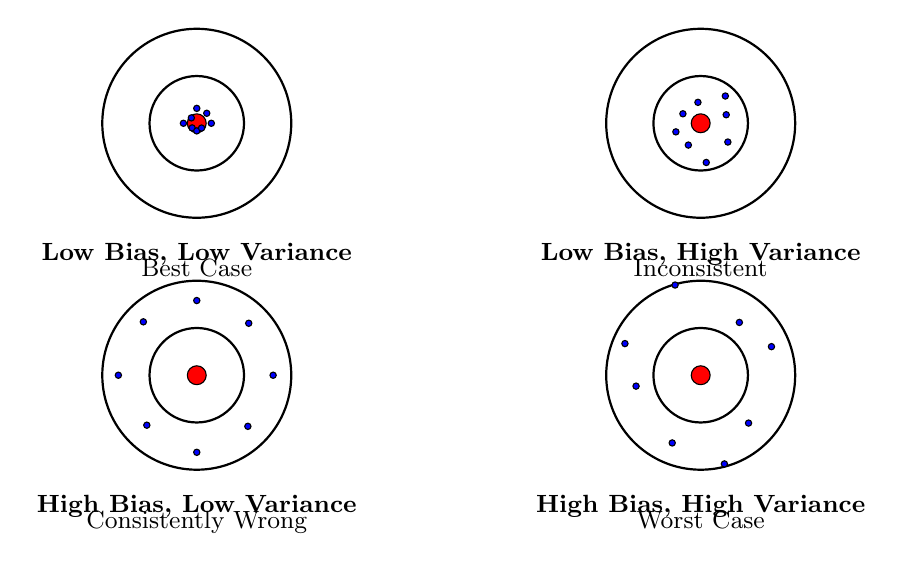
\begin{tikzpicture}[scale=0.4]
% Low Bias, Low Variance (top left)
\begin{scope}[xshift=-8cm, yshift=4cm]
  \draw[thick] (0,0) circle (3);
  \draw[thick] (0,0) circle (1.5);
  \draw[fill=red] (0,0) circle (0.3);
  % Tight cluster near center
  \foreach \i in {1,...,8} {
    \pgfmathsetmacro{\angle}{45*\i}
    \pgfmathsetmacro{\radius}{0.2 + 0.3*rnd}
    \draw[fill=blue] (\angle:\radius) circle (0.1);
  }
  \node[below] at (0,-3.5) {\small \textbf{Low Bias, Low Variance}};
  \node[below] at (0,-4) {\small Best Case};
\end{scope}

% Low Bias, High Variance (top right)
\begin{scope}[xshift=8cm, yshift=4cm]
  \draw[thick] (0,0) circle (3);
  \draw[thick] (0,0) circle (1.5);
  \draw[fill=red] (0,0) circle (0.3);
  % Scattered around center
  \foreach \i in {1,...,8} {
    \pgfmathsetmacro{\angle}{45*\i + 20*rnd}
    \pgfmathsetmacro{\radius}{0.5 + 1.2*rnd}
    \draw[fill=blue] (\angle:\radius) circle (0.1);
  }
  \node[below] at (0,-3.5) {\small \textbf{Low Bias, High Variance}};
  \node[below] at (0,-4) {\small Inconsistent};
\end{scope}

% High Bias, Low Variance (bottom left)
\begin{scope}[xshift=-8cm, yshift=-4cm]
  \draw[thick] (0,0) circle (3);
  \draw[thick] (0,0) circle (1.5);
  \draw[fill=red] (0,0) circle (0.3);
  % Tight cluster away from center
  \foreach \i in {1,...,8} {
    \pgfmathsetmacro{\angle}{45*\i}
    \pgfmathsetmacro{\radius}{2.2 + 0.3*rnd}
    \draw[fill=blue] (\angle:\radius) circle (0.1);
  }
  \node[below] at (0,-3.5) {\small \textbf{High Bias, Low Variance}};
  \node[below] at (0,-4) {\small Consistently Wrong};
\end{scope}

% High Bias, High Variance (bottom right)
\begin{scope}[xshift=8cm, yshift=-4cm]
  \draw[thick] (0,0) circle (3);
  \draw[thick] (0,0) circle (1.5);
  \draw[fill=red] (0,0) circle (0.3);
  % Scattered away from center
  \foreach \i in {1,...,8} {
    \pgfmathsetmacro{\angle}{45*\i + 30*rnd}
    \pgfmathsetmacro{\radius}{2.0 + 1.0*rnd}
    \draw[fill=blue] (\angle:\radius) circle (0.1);
  }
  \node[below] at (0,-3.5) {\small \textbf{High Bias, High Variance}};
  \node[below] at (0,-4) {\small Worst Case};
\end{scope}
\end{tikzpicture}
\end{center}

\textbf{Key:} Red = True target, Blue dots = Predictions across different training sets
\end{frame}

\begin{frame}{Mathematical Foundation: Bias-Variance Decomposition}
\begin{definitionbox}{The Fundamental Equation}
For any learning algorithm, the expected prediction error can be decomposed as:
$$\text{Expected Error} = \text{Bias}^2 + \text{Variance} + \text{Irreducible Error}$$
\end{definitionbox}

Where:
\begin{itemize}
\item $\text{Bias}^2 = (\mathbb{E}[\hat{f}(x)] - f(x))^2$ \\
  \textit{Squared difference between average prediction and true function}
\item $\text{Variance} = \mathbb{E}[(\hat{f}(x) - \mathbb{E}[\hat{f}(x)])^2]$ \\
  \textit{Expected squared deviation from average prediction}
\item $\text{Irreducible Error} = \sigma^2$ \\
  \textit{Noise in the data that no model can eliminate}
\end{itemize}
\end{frame}

\begin{frame}{Intuitive Understanding of Each Component}
\begin{examplebox}{Bias: "Are we systematically wrong?"}
\begin{itemize}
\item High Bias: Linear model fitting curved data
\item Low Bias: Flexible model that can approximate true function
\item \textbf{Think}: Average error if we could train on infinite datasets
\end{itemize}
\end{examplebox}

\begin{examplebox}{Variance: "Are we consistently wrong?"}
\begin{itemize}
\item High Variance: Model predictions change drastically with new training data
\item Low Variance: Model predictions remain stable across different datasets
\item \textbf{Think}: How much do predictions fluctuate between training runs?
\end{itemize}
\end{examplebox}

\textbf{Key Insight:} Both contribute to total error, but reducing one often increases the other!
\end{frame}

	\begin{frame}{An example}
	Consider the dataset below
	\begin{figure}[h]
	    \centering
	    \begin{minipage}{0.45\textwidth}
	        \centering
	        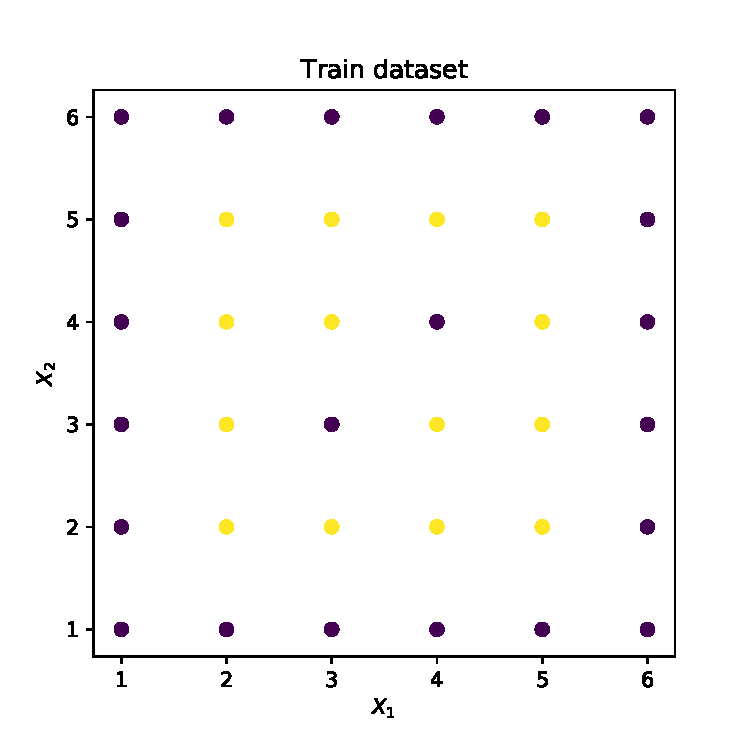
\includegraphics[width=\textwidth]{dataset-2-train}
	        \caption{Train Set}
	    \end{minipage}
	    \hfill
	    \begin{minipage}{0.45\textwidth}
	        \centering
	        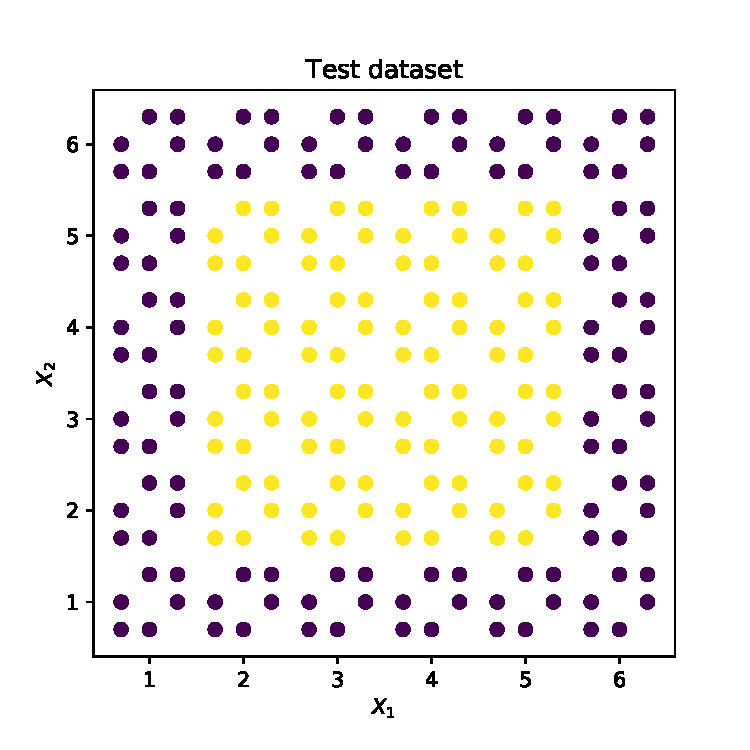
\includegraphics[width=\textwidth]{dataset-2-test}
	        \caption{Test Set}
	    \end{minipage}
	\end{figure}
	\end{frame}


\begin{frame}{High Bias Example: Medical Diagnosis}
\begin{examplebox}{Oversimplified Medical Model}
\textbf{Model}: "All patients with fever have flu"
\begin{itemize}
\item High Bias: Ignores other symptoms, medical history
\item Systematic Error: Misses pneumonia, COVID, etc.
\item Poor Performance: Wrong diagnoses even with more data
\end{itemize}
\end{examplebox}

\begin{keypointsbox}
\textbf{Solution:} Increase model complexity, add features, use more flexible algorithms
\end{keypointsbox}
\end{frame}

\begin{frame}{High Bias Example: Financial Prediction}
\begin{examplebox}{Oversimplified Stock Model}
\textbf{Model}: "Stock price only depends on previous day's price"
\begin{itemize}
\item High Bias: Ignores market conditions, company news, economic indicators
\item Systematic Error: Misses major trend changes
\item Poor Performance: Consistently wrong about market direction
\end{itemize}
\end{examplebox}

\begin{keypointsbox}
\textbf{Key Insight:} High bias models have systematic blind spots that more data cannot fix
\end{keypointsbox}
\end{frame}


\begin{frame}{High Variance Example: Image Recognition}
\begin{examplebox}{Overcomplicated Vision Model}
\textbf{Model}: Deep network with 1000 layers on small dataset
\begin{itemize}
\item High Variance: Different training sets → completely different filters
\item Memorization: Learns specific pixel patterns, not object features
\item Poor Generalization: Fails on slightly different images
\end{itemize}
\end{examplebox}

\begin{keypointsbox}
\textbf{Solution:} Reduce model complexity, regularization, more training data
\end{keypointsbox}
\end{frame}

\begin{frame}{High Variance Example: Text Classification}
\begin{examplebox}{Overcomplicated Text Model}
\textbf{Model}: Memorizing entire sentences instead of key words
\begin{itemize}
\item High Variance: Adding one new training email changes all predictions
\item Memorization: Learns exact phrases, not semantic meaning
\item Poor Generalization: Fails on paraphrased or slightly different text
\end{itemize}
\end{examplebox}

\begin{keypointsbox}
\textbf{Key Insight:} High variance models are too sensitive to training data variations
\end{keypointsbox}
\end{frame}


	\begin{frame}{Intuition for Variance}
	A small change in data can lead to very different models.\\
	\vspace{1cm}
	\begin{columns}
		\begin{column}{0.5\textwidth}{\hspace{1.75cm} Dataset 1}
			\begin{center}
			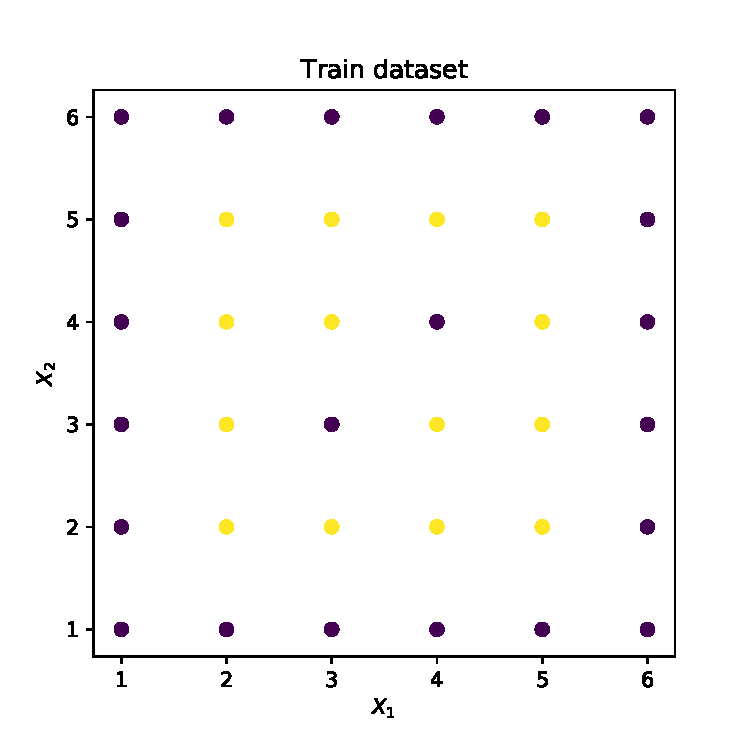
\includegraphics[width = \textwidth]{dataset-2-train}
			\end{center}
		\end{column}
		\begin{column}{0.5\textwidth}{\hspace{1.75cm} Dataset 2}
			\begin{center}
			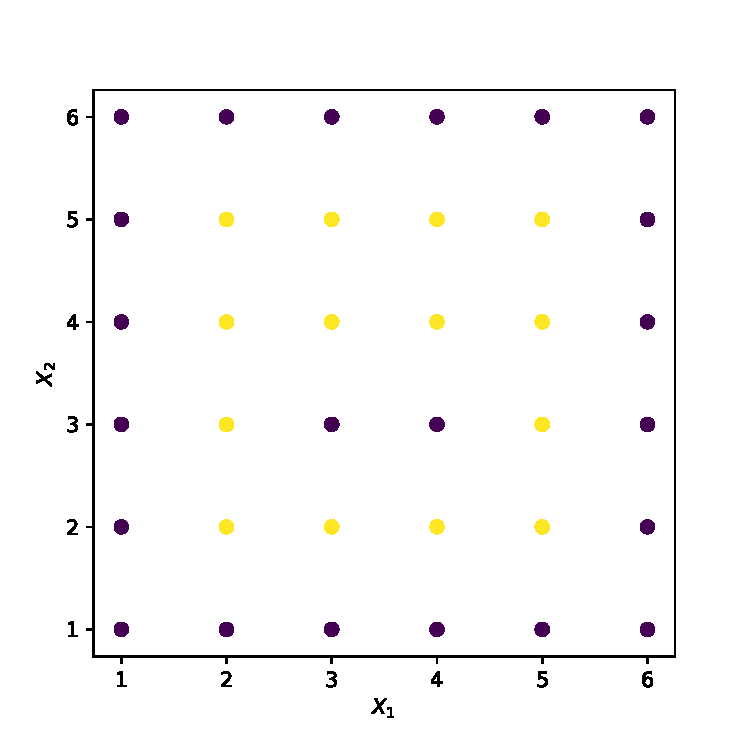
\includegraphics[width = \textwidth]{dataset-2-train-var}
			\end{center}
		\end{column}
	\end{columns}
	\end{frame}


	\begin{frame}{Intuition for Variance}
	\begin{columns}
		\begin{column}{0.5\textwidth}
			\begin{center}
			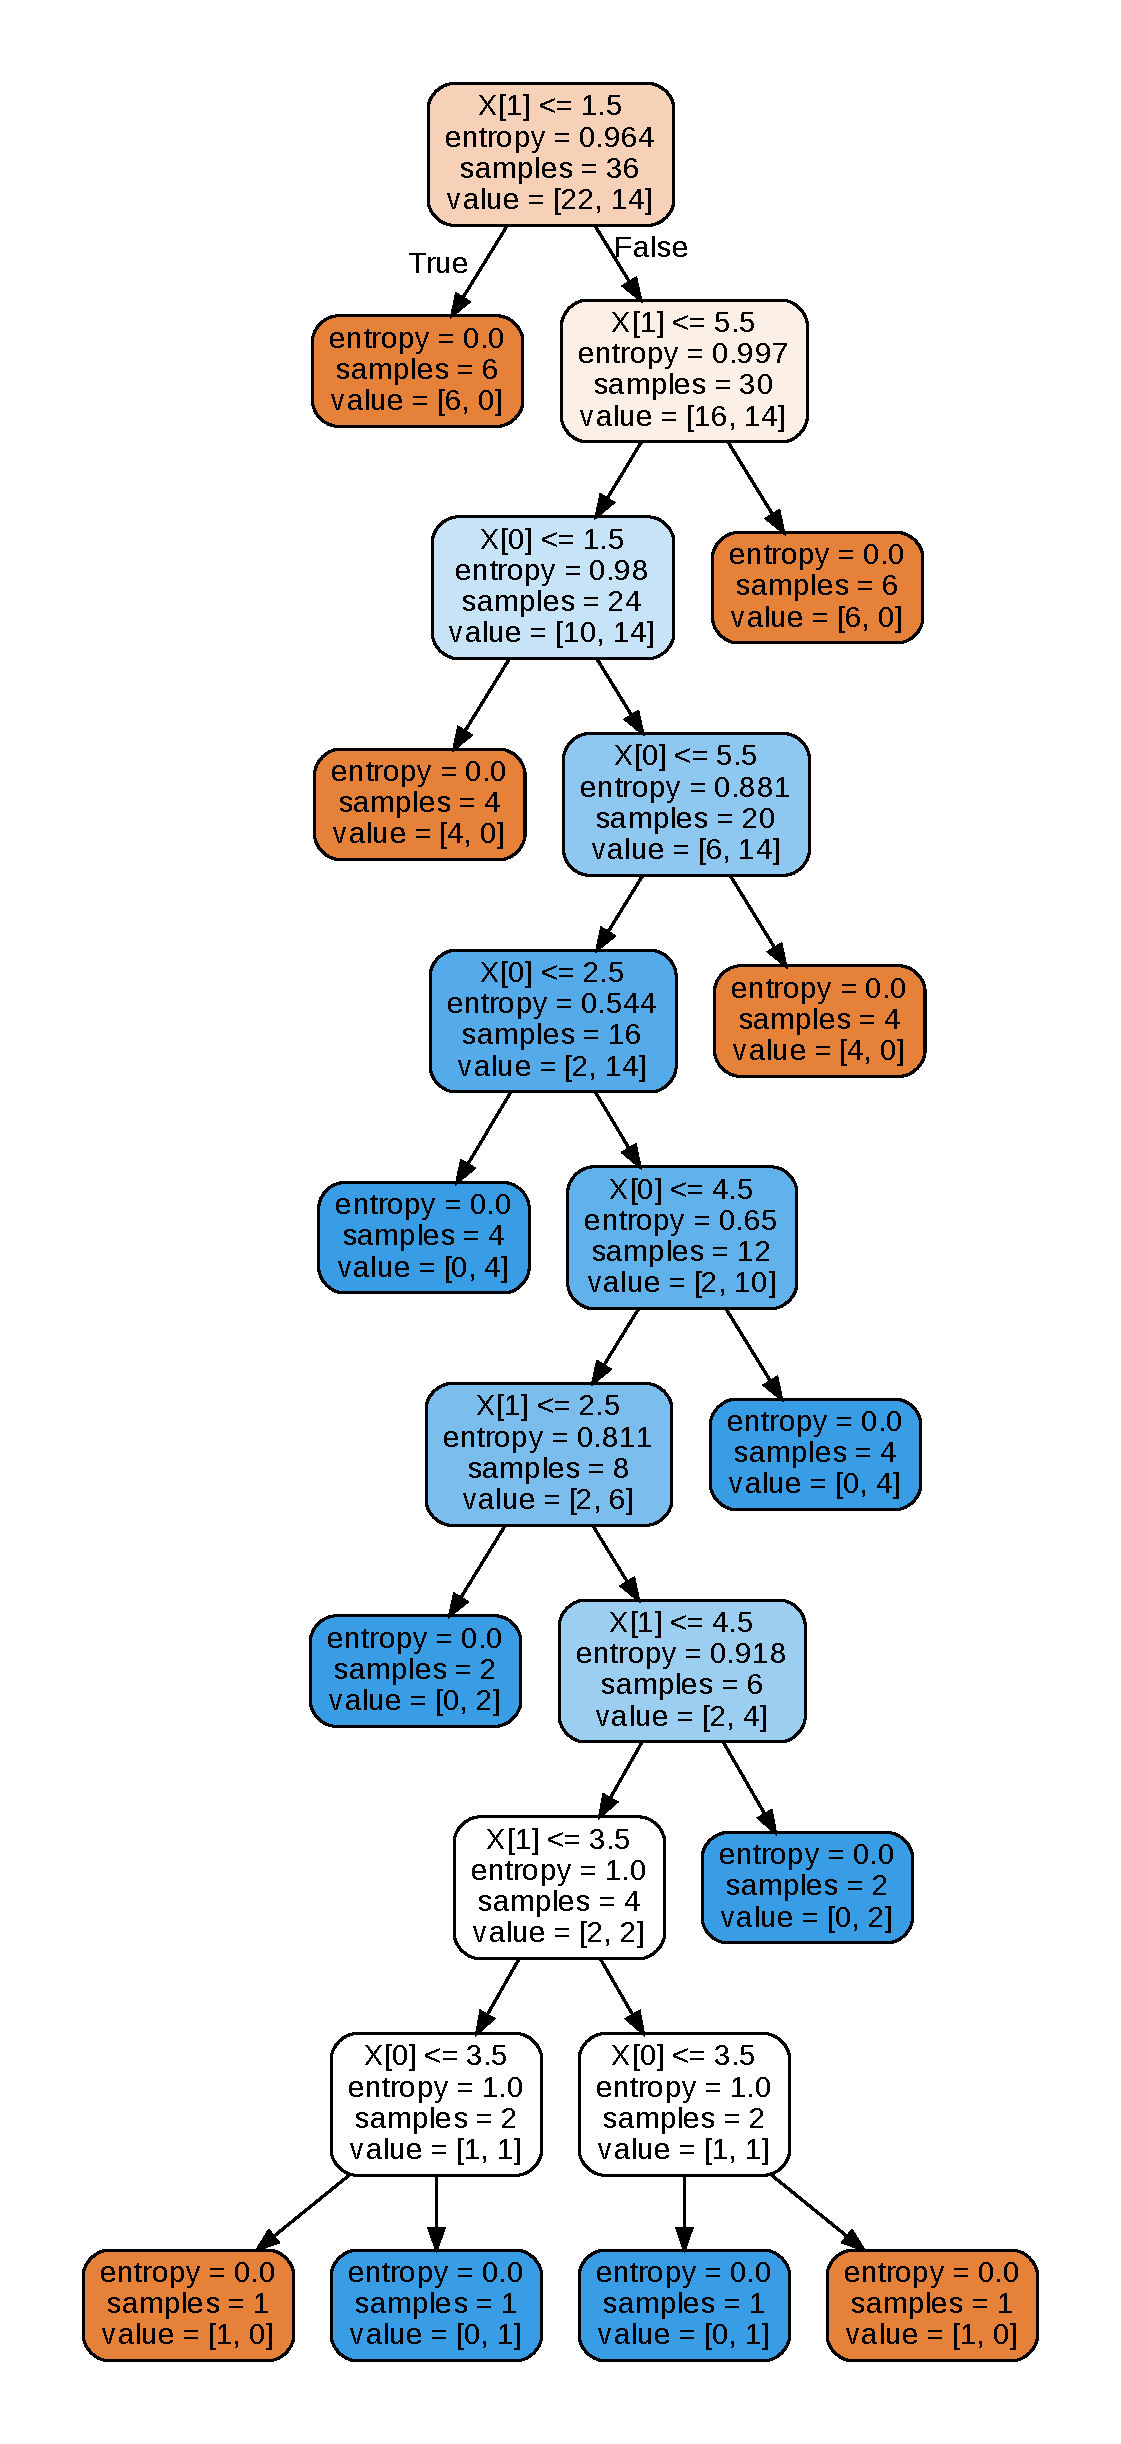
\includegraphics[scale=0.2]{var_1}
			\end{center}
		\end{column}
		\begin{column}{0.5\textwidth}
			\begin{center}
			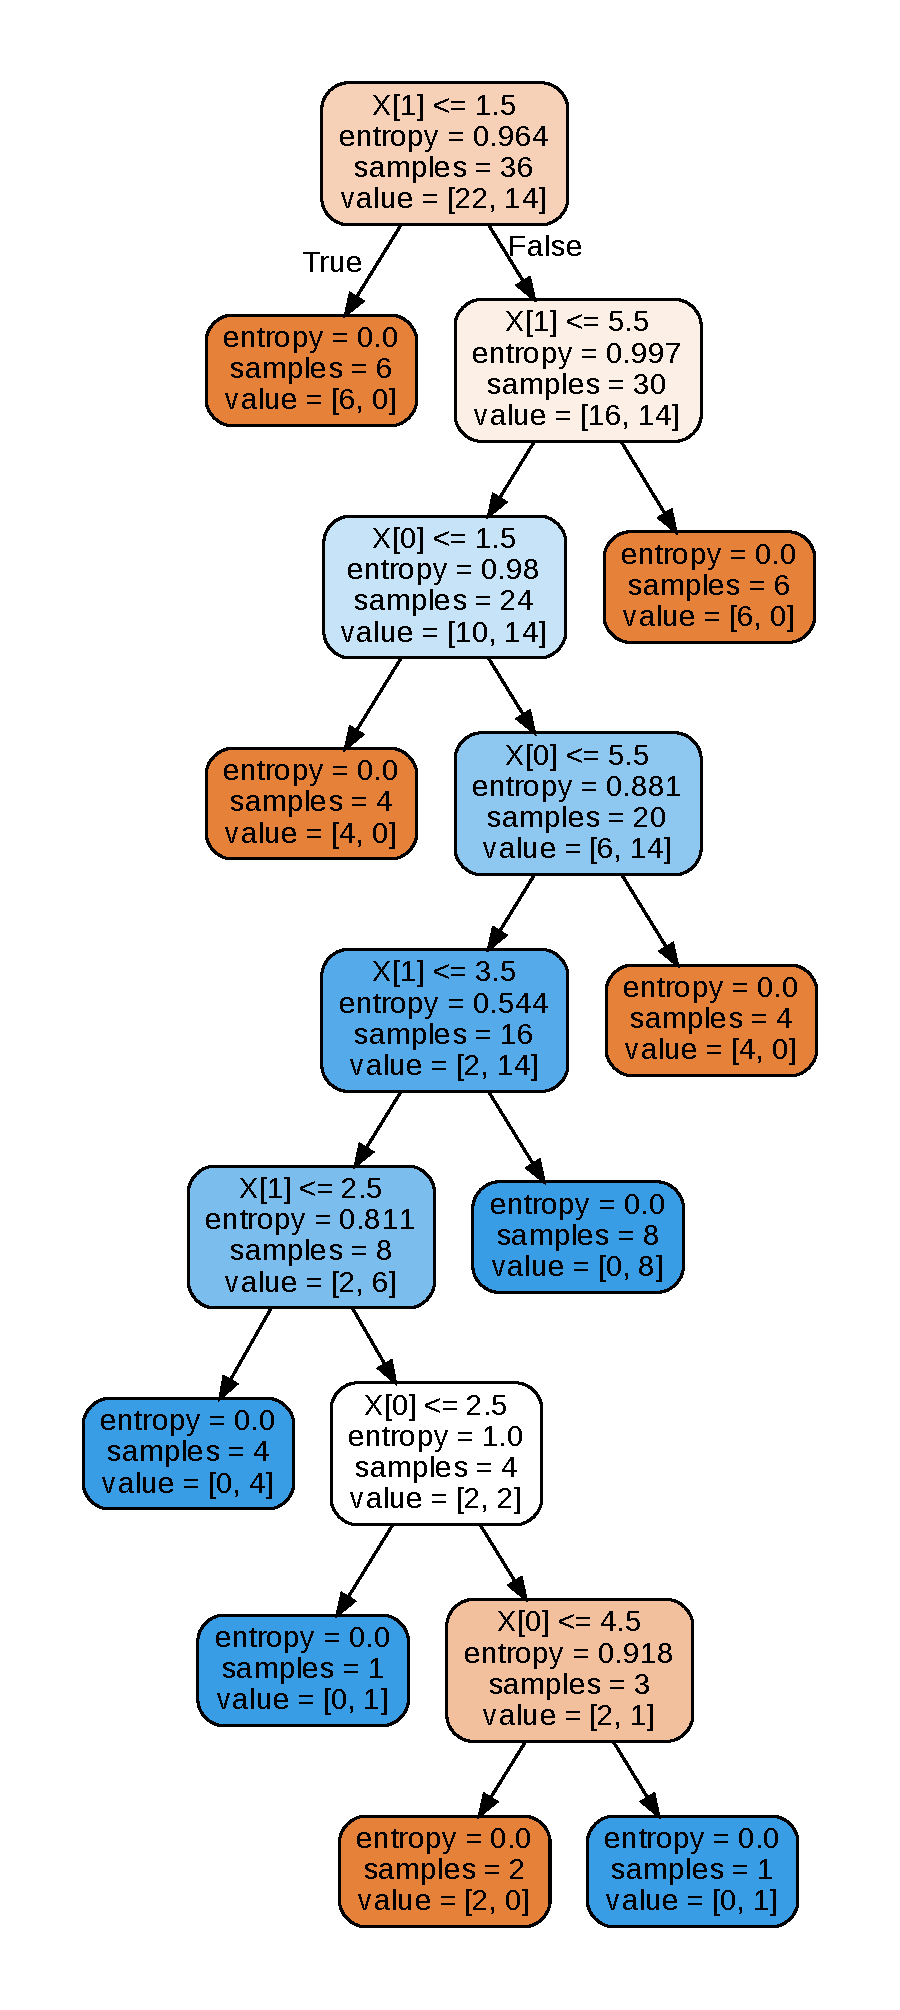
\includegraphics[scale=0.2]{var_2}
			\end{center}
		\end{column}
	\end{columns}
	\end{frame}

\begin{frame}{The Bias-Variance Tradeoff Visualized}
\begin{examplebox}{The Fundamental Tradeoff}
\begin{itemize}
\item \textbf{Increase Model Complexity}:
  \begin{itemize}
  \item Bias ↓ (can fit more complex patterns)
  \item Variance ↑ (more sensitive to training data)
  \end{itemize}
\item \textbf{Decrease Model Complexity}:
  \begin{itemize}
  \item Bias ↑ (makes stronger assumptions)
  \item Variance ↓ (more stable predictions)
  \end{itemize}
\end{itemize}
\end{examplebox}

\begin{keypointsbox}
\textbf{The Sweet Spot:}
Find the complexity that minimizes: $\text{Bias}^2 + \text{Variance} + \text{Noise}$
\end{keypointsbox}

\textbf{Different algorithms have different bias-variance profiles!}
\end{frame}

\begin{frame}{Comparing Algorithms: Bias-Variance Profiles}
\begin{definitionbox}{Algorithm Characteristics}
\begin{itemize}
\item \textbf{k-NN with small k}: Low bias, high variance
\item \textbf{k-NN with large k}: High bias, low variance
\item \textbf{Linear Regression}: High bias, low variance
\item \textbf{Deep Neural Networks}: Low bias, high variance (without regularization)
\item \textbf{Decision Trees}: Low bias, high variance
\item \textbf{Random Forest}: Lower variance than single trees
\end{itemize}
\end{definitionbox}

\textbf{Key Insight:} No single algorithm is best for all problems!
\end{frame}


	\begin{frame}{A Good Fit: Finding the Sweet Spot}
	\begin{columns}
		\begin{column}{0.5\textwidth}
			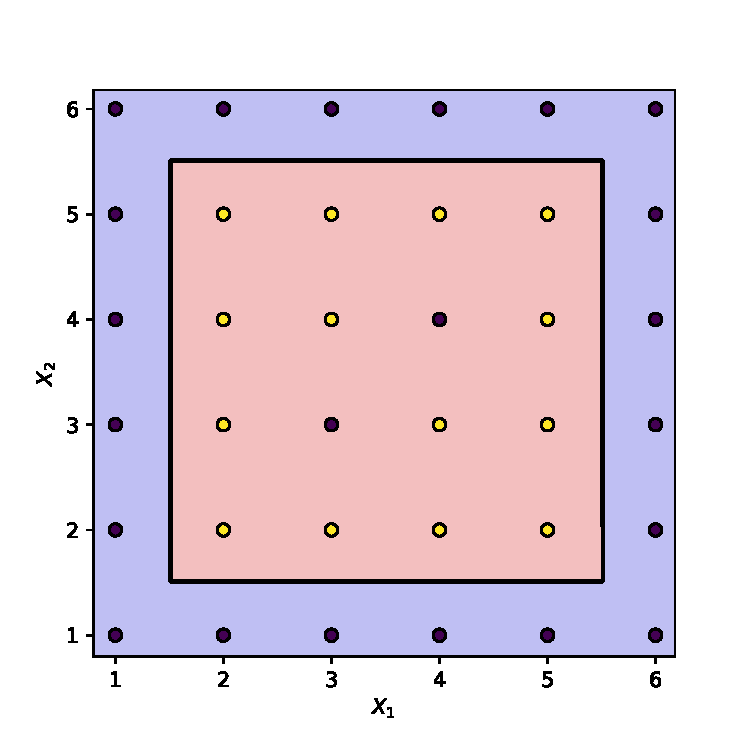
\includegraphics[width=\textwidth]{example-2-optimal-boundary}
		\end{column}
		\begin{column}{0.5\textwidth}
			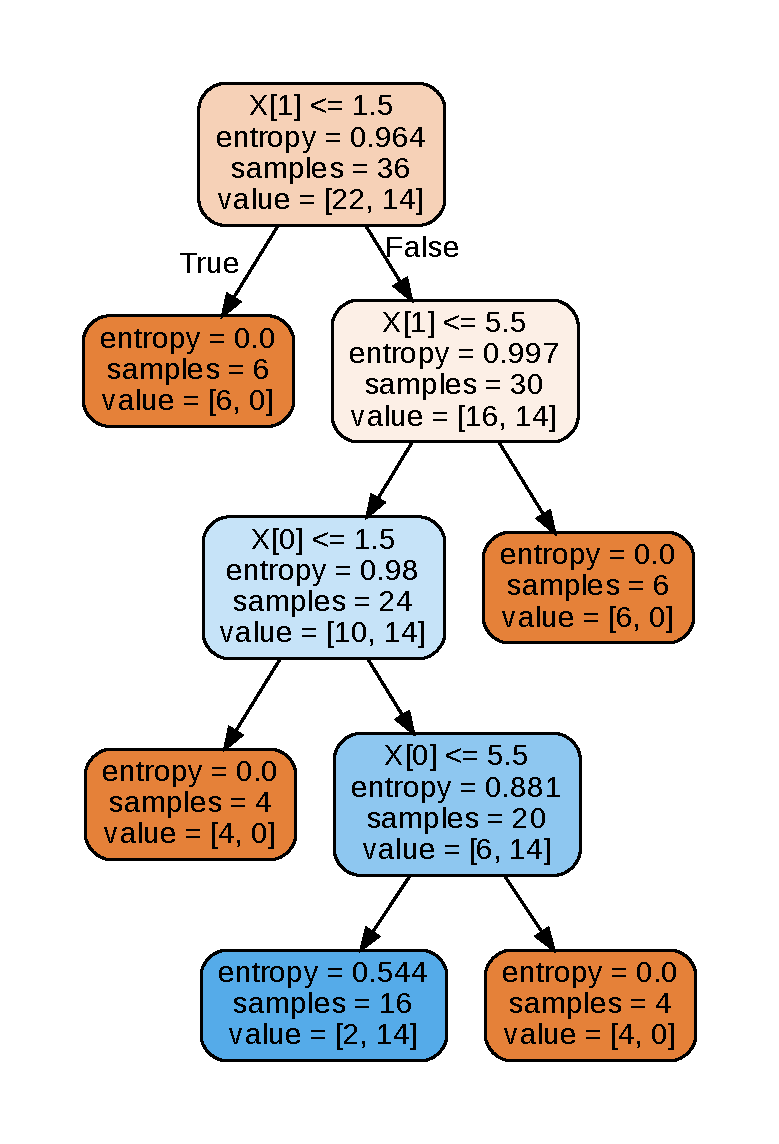
\includegraphics[width =\textwidth]{example-2-optimal-tree}
		\end{column}
	\end{columns}

	\end{frame}

	\begin{frame}{Accuracy vs Depth Curve}
		\begin{center}
		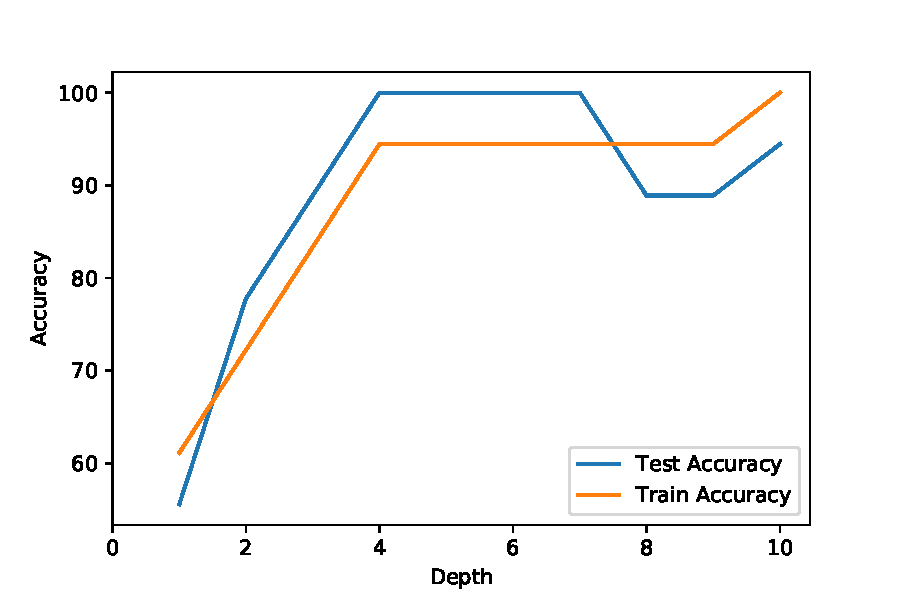
\includegraphics[scale=0.55]{acc-depth-plot}
	\end{center}
	\pause As depth increases, train accuracy improves\\
	\pause As depth increases, test accuracy improves till a point\\
	\pause At very high depths, test accuracy is not good (overfitting). 

	\end{frame}

	\begin{frame}{Accuracy vs Depth: Understanding All Three Regions}
	\begin{center}
	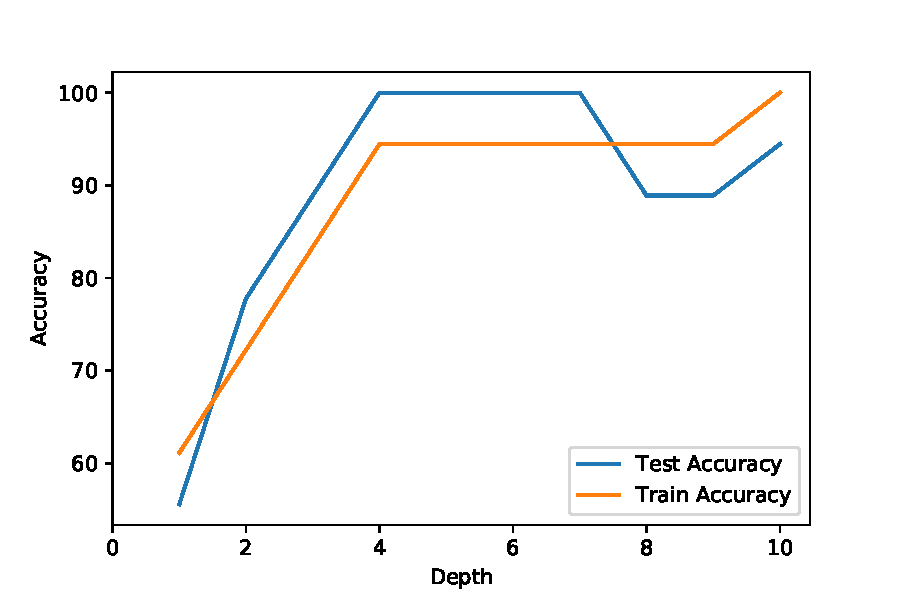
\includegraphics[scale=0.5]{acc-depth-plot}
	\end{center}
	
	\begin{keypointsbox}
	\textbf{Three Key Regions:}
	\begin{itemize}
	\item \textbf{Underfitting}: Too simple models, poor performance on both training and test
	\item \textbf{Good Fit}: Optimal complexity, best test accuracy
	\item \textbf{Overfitting}: Too complex models, learns noise from training data
	\end{itemize}
	\end{keypointsbox}
	\end{frame}

\begin{frame}{The Complete Picture: Bias-Variance Through Model Complexity}
\begin{center}
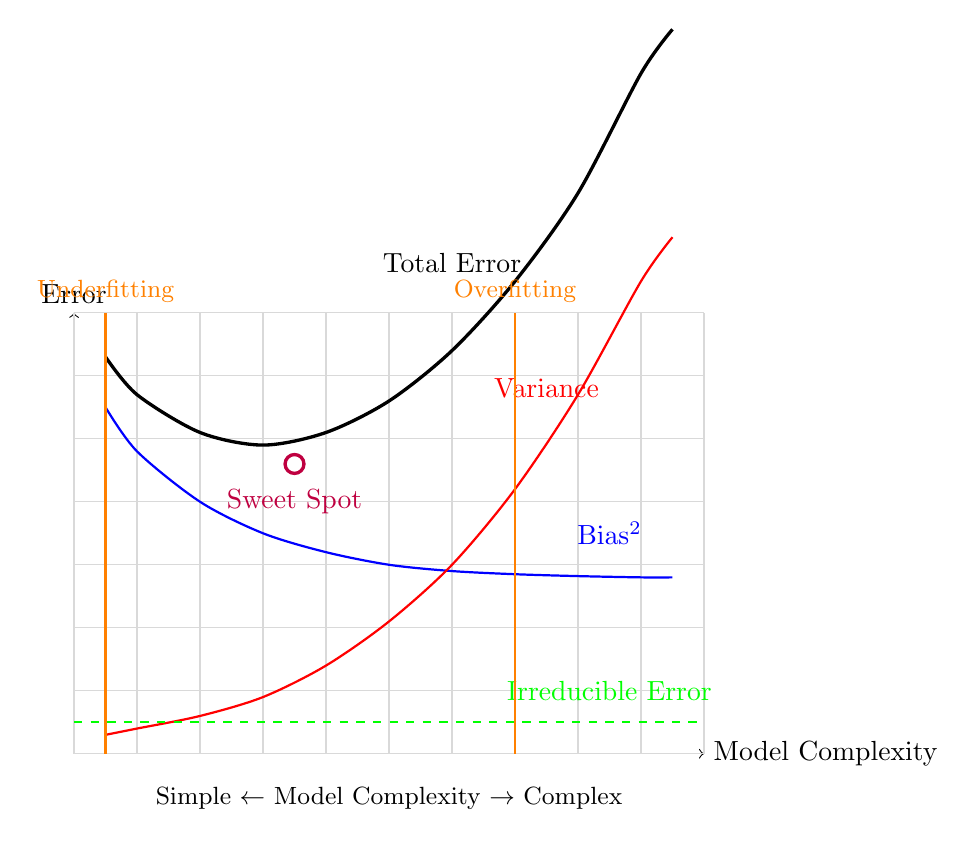
\begin{tikzpicture}[scale=0.8]
    % Axes
    \draw[->] (0,0) -- (10,0) node[right] {Model Complexity};
    \draw[->] (0,0) -- (0,7) node[above] {Error};
    
    % Grid
    \draw[gray!30] (0,0) grid (10,7);
    
    % Bias curve (decreasing)
    \draw[blue, thick, smooth] plot coordinates {
        (0.5,5.5) (1,4.8) (2,4.0) (3,3.5) (4,3.2) (5,3.0) (6,2.9) (7,2.85) (8,2.82) (9,2.8) (9.5,2.8)
    };
    \node[blue] at (8.5,3.5) {Bias$^2$};
    
    % Variance curve (increasing)
    \draw[red, thick, smooth] plot coordinates {
        (0.5,0.3) (1,0.4) (2,0.6) (3,0.9) (4,1.4) (5,2.1) (6,3.0) (7,4.2) (8,5.7) (9,7.5) (9.5,8.2)
    };
    \node[red] at (7.5,5.8) {Variance};
    
    % Total error curve (U-shaped)
    \draw[black, very thick, smooth] plot coordinates {
        (0.5,6.3) (1,5.7) (2,5.1) (3,4.9) (4,5.1) (5,5.6) (6,6.4) (7,7.5) (8,8.9) (9,10.8) (9.5,11.5)
    };
    \node[black] at (6,7.8) {Total Error};
    
    % Irreducible error (constant)
    \draw[green, thick, dashed] (0,0.5) -- (10,0.5);
    \node[green] at (8.5,1) {Irreducible Error};
    
    % Optimal point
    \draw[purple, very thick] (3.5,4.6) circle (0.15);
    \node[purple] at (3.5,4) {Sweet Spot};
    
    % Regions
    \draw[orange, thick] (0.5,0) -- (0.5,7) node[above] {\small Underfitting};
    \draw[orange, thick] (7,0) -- (7,7) node[above] {\small Overfitting};
    
    % Labels
    \node at (5,-0.7) {\small Simple $\leftarrow$ Model Complexity $\rightarrow$ Complex};
\end{tikzpicture}
\end{center}

\begin{keypointsbox}
\textbf{Key Insight:} The optimal complexity minimizes total error, balancing bias and variance
\end{keypointsbox}
\end{frame}

\begin{frame}{Underfitting Visualized: When Models Are Too Simple}
\begin{columns}
\begin{column}{0.6\textwidth}
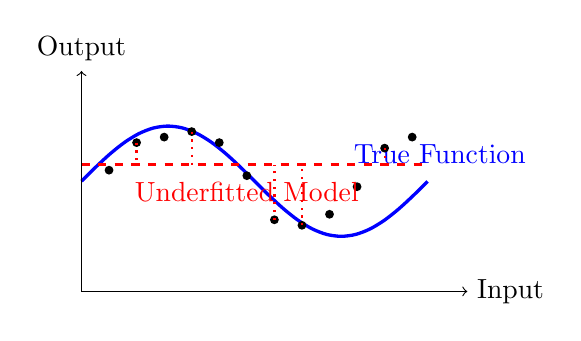
\begin{tikzpicture}[scale=0.7]
    % True function (sine wave)
    \draw[domain=0:6.28, smooth, variable=\x, blue, very thick] plot ({\x}, {2 + sin(\x r)});
    \node[blue] at (6.5, 2.5) {True Function};
    
    % Data points with noise
    \foreach \x/\y in {0.5/2.2, 1/2.7, 1.5/2.8, 2/2.9, 2.5/2.7, 3/2.1, 3.5/1.3, 4/1.2, 4.5/1.4, 5/1.9, 5.5/2.6, 6/2.8} {
        \fill[black] (\x,\y) circle (0.08);
    }
    
    % Underfitting line (constant)
    \draw[red, very thick, dashed] (0,2.3) -- (6.28,2.3);
    \node[red] at (3, 1.8) {Underfitted Model};
    
    % Axes
    \draw[->] (0,0) -- (7,0) node[right] {Input};
    \draw[->] (0,0) -- (0,4) node[above] {Output};
    
    % Error illustration
    \foreach \x/\y in {1/2.7, 2/2.9, 3.5/1.3, 4/1.2, 5.5/2.6} {
        \draw[red, dotted, thick] (\x,\y) -- (\x,2.3);
    }
\end{tikzpicture}
\end{column}
\begin{column}{0.4\textwidth}
\begin{alertbox}{High Bias Problem}
\begin{itemize}
\item \textbf{Model}: Too simple (constant)
\item \textbf{Assumption}: "Output never changes"
\item \textbf{Result}: Systematic error
\item \textbf{Training Error}: High
\item \textbf{Test Error}: High
\end{itemize}
\end{alertbox}

\textbf{Solution:} Increase model complexity
\end{column}
\end{columns}
\end{frame}

\begin{frame}{Overfitting Visualized: When Models Are Too Complex}
\begin{columns}
\begin{column}{0.6\textwidth}
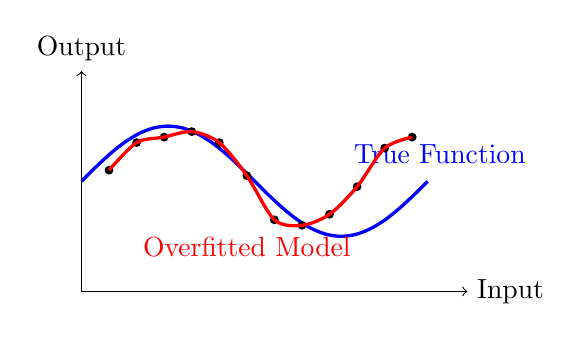
\begin{tikzpicture}[scale=0.7]
    % True function (sine wave)
    \draw[domain=0:6.28, smooth, variable=\x, blue, very thick] plot ({\x}, {2 + sin(\x r)});
    \node[blue] at (6.5, 2.5) {True Function};
    
    % Data points with noise
    \foreach \x/\y in {0.5/2.2, 1/2.7, 1.5/2.8, 2/2.9, 2.5/2.7, 3/2.1, 3.5/1.3, 4/1.2, 4.5/1.4, 5/1.9, 5.5/2.6, 6/2.8} {
        \fill[black] (\x,\y) circle (0.08);
    }
    
    % Overfitting curve (goes through all points)
    \draw[red, very thick] plot[smooth] coordinates {
        (0.5,2.2) (1,2.7) (1.5,2.8) (2,2.9) (2.5,2.7) (3,2.1) (3.5,1.3) (4,1.2) (4.5,1.4) (5,1.9) (5.5,2.6) (6,2.8)
    };
    \node[red] at (3, 0.8) {Overfitted Model};
    
    % Axes
    \draw[->] (0,0) -- (7,0) node[right] {Input};
    \draw[->] (0,0) -- (0,4) node[above] {Output};
\end{tikzpicture}
\end{column}
\begin{column}{0.4\textwidth}
\begin{alertbox}{High Variance Problem}
\begin{itemize}
\item \textbf{Model}: Too complex (memorizes)
\item \textbf{Assumption}: "Fit every data point exactly"
\item \textbf{Result}: Learns noise
\item \textbf{Training Error}: Very low
\item \textbf{Test Error}: High
\end{itemize}
\end{alertbox}

\textbf{Solution:} Reduce complexity or regularize
\end{column}
\end{columns}
\end{frame}

\begin{frame}{Good Fit: The Sweet Spot}
\begin{columns}
\begin{column}{0.6\textwidth}
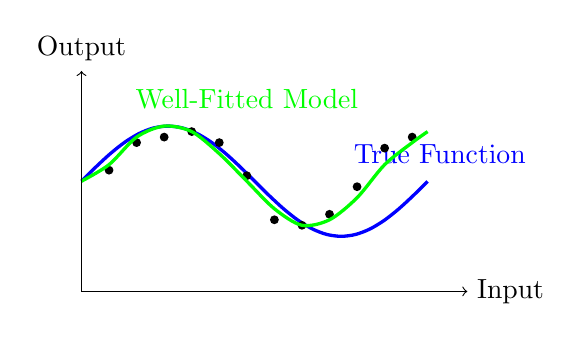
\begin{tikzpicture}[scale=0.7]
    % True function (sine wave)
    \draw[domain=0:6.28, smooth, variable=\x, blue, very thick] plot ({\x}, {2 + sin(\x r)});
    \node[blue] at (6.5, 2.5) {True Function};
    
    % Data points with noise
    \foreach \x/\y in {0.5/2.2, 1/2.7, 1.5/2.8, 2/2.9, 2.5/2.7, 3/2.1, 3.5/1.3, 4/1.2, 4.5/1.4, 5/1.9, 5.5/2.6, 6/2.8} {
        \fill[black] (\x,\y) circle (0.08);
    }
    
    % Good fit curve (smooth approximation)
    \draw[green, very thick] plot[smooth] coordinates {
        (0,2.0) (0.5,2.3) (1,2.8) (1.5,3.0) (2,2.9) (2.5,2.5) (3,2.0) (3.5,1.5) (4,1.2) (4.5,1.3) (5,1.7) (5.5,2.3) (6,2.7) (6.28,2.9)
    };
    \node[green] at (3, 3.5) {Well-Fitted Model};
    
    % Axes
    \draw[->] (0,0) -- (7,0) node[right] {Input};
    \draw[->] (0,0) -- (0,4) node[above] {Output};
\end{tikzpicture}
\end{column}
\begin{column}{0.4\textwidth}
\begin{examplebox}{Goldilocks Principle}
\begin{itemize}
\item \textbf{Model}: Just right complexity
\item \textbf{Result}: Good generalization
\item \textbf{Errors}: Training moderate, test low
\end{itemize}
\end{examplebox}
\end{column}
\end{columns}
\end{frame}

\begin{frame}{Interactive Example: Polynomial Fitting}
\begin{center}
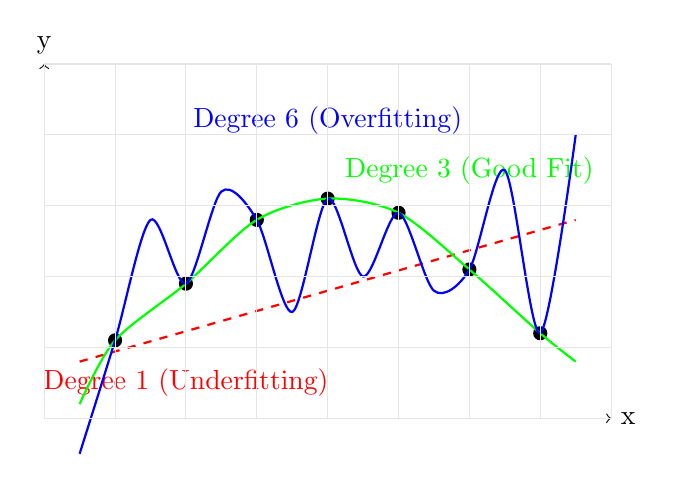
\begin{tikzpicture}[scale=0.9]
    % Data points
    \foreach \x/\y in {1/1.1, 2/1.9, 3/2.8, 4/3.1, 5/2.9, 6/2.1, 7/1.2} {
        \fill[black] (\x,\y) circle (0.1);
    }
    
    % Degree 1 polynomial (underfitting)
    \draw[red, thick, dashed] (0.5,0.8) -- (7.5,2.8);
    \node[red] at (2,0.5) {Degree 1 (Underfitting)};
    
    % Degree 3 polynomial (good fit)
    \draw[green, thick] plot[smooth] coordinates {
        (0.5,0.2) (1,1.1) (2,1.9) (3,2.8) (4,3.1) (5,2.9) (6,2.1) (7,1.2) (7.5,0.8)
    };
    \node[green] at (6,3.5) {Degree 3 (Good Fit)};
    
    % Degree 6 polynomial (overfitting)
    \draw[blue, thick] plot[smooth] coordinates {
        (0.5,-0.5) (1,1.1) (1.5,2.8) (2,1.9) (2.5,3.2) (3,2.8) (3.5,1.5) (4,3.1) (4.5,2.0) (5,2.9) (5.5,1.8) (6,2.1) (6.5,3.5) (7,1.2) (7.5,4.0)
    };
    \node[blue] at (4,4.2) {Degree 6 (Overfitting)};
    
    % Axes
    \draw[->] (0,0) -- (8,0) node[right] {x};
    \draw[->] (0,0) -- (0,5) node[above] {y};
    
    % Grid
    \draw[gray!20] (0,0) grid (8,5);
\end{tikzpicture}
\end{center}

\textbf{Question:} Which polynomial would you choose and why?
\end{frame}

	\begin{frame}{The big question!?}
	\only<1-2>{
	How to find the optimal depth for a decision tree?\\
	}
	\only<2>{
	\vspace{1cm}
	Use cross-validation!
	}
	\end{frame}

\begin{frame}{The Problem: How Do We Find the Sweet Spot?}
\begin{alertbox}{The Fundamental Challenge}
\begin{itemize}
\item Can't use test data to select model complexity (that's cheating!)
\item Can't trust training error (always decreases with complexity)
\item Need unbiased estimate of generalization performance
\end{itemize}
\end{alertbox}

\begin{keypointsbox}
\textbf{Solution:} Cross-validation provides honest estimates of generalization!
\end{keypointsbox}
\end{frame}

\begin{frame}{Why Training Error Fails for Model Selection}
\begin{examplebox}{Training Error is Optimistically Biased}
\begin{itemize}
\item Complex models: Training error $\approx 0$, but test error is high
\item Simple models: Training error is high, test error might be high too
\item Training error systematically underestimates true error
\end{itemize}
\end{examplebox}

\begin{keypointsbox}
\textbf{Key Insight:} Models that fit training data perfectly often fail on new data
\end{keypointsbox}
\end{frame}

\begin{frame}{Cross-Validation: The Core Idea}
\begin{definitionbox}{The Philosophy}
Simulate having multiple independent test sets by:
\begin{enumerate}
\item Split training data into multiple folds
\item Train on some folds, validate on others
\item Rotate which folds are used for validation
\item Average the validation performance
\end{enumerate}
\end{definitionbox}
\end{frame}

\begin{frame}{Benefits of Cross-Validation}
\begin{keypointsbox}
\textbf{Key Benefits:}
\begin{itemize}
\item Uses all data for both training and validation
\item Provides robust estimates vs single train/validation split
\item Reduces dependence on particular data split
\item Helps detect overfitting to validation set
\end{itemize}
\end{keypointsbox}

\begin{alertbox}{Important}
Cross-validation gives us honest estimates for model selection!
\end{alertbox}
\end{frame}


	\begin{frame}{Our General Training Flow}
	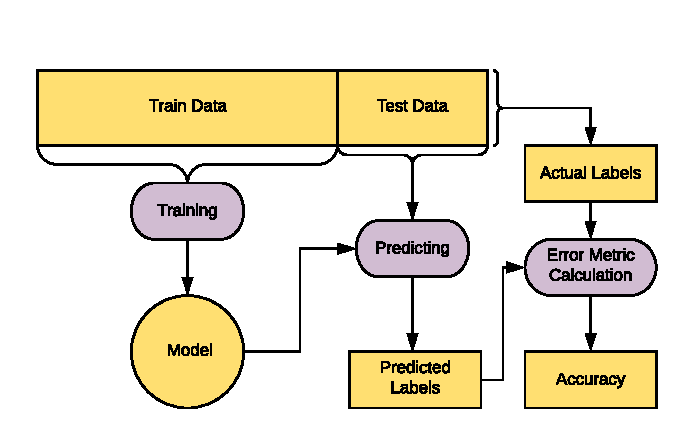
\includegraphics[width = \textwidth]{../assets/bias-variance/diagrams/general-workflow}
	\end{frame}

	\begin{frame}{K-Fold cross-validation: Utilise full dataset for testing}
	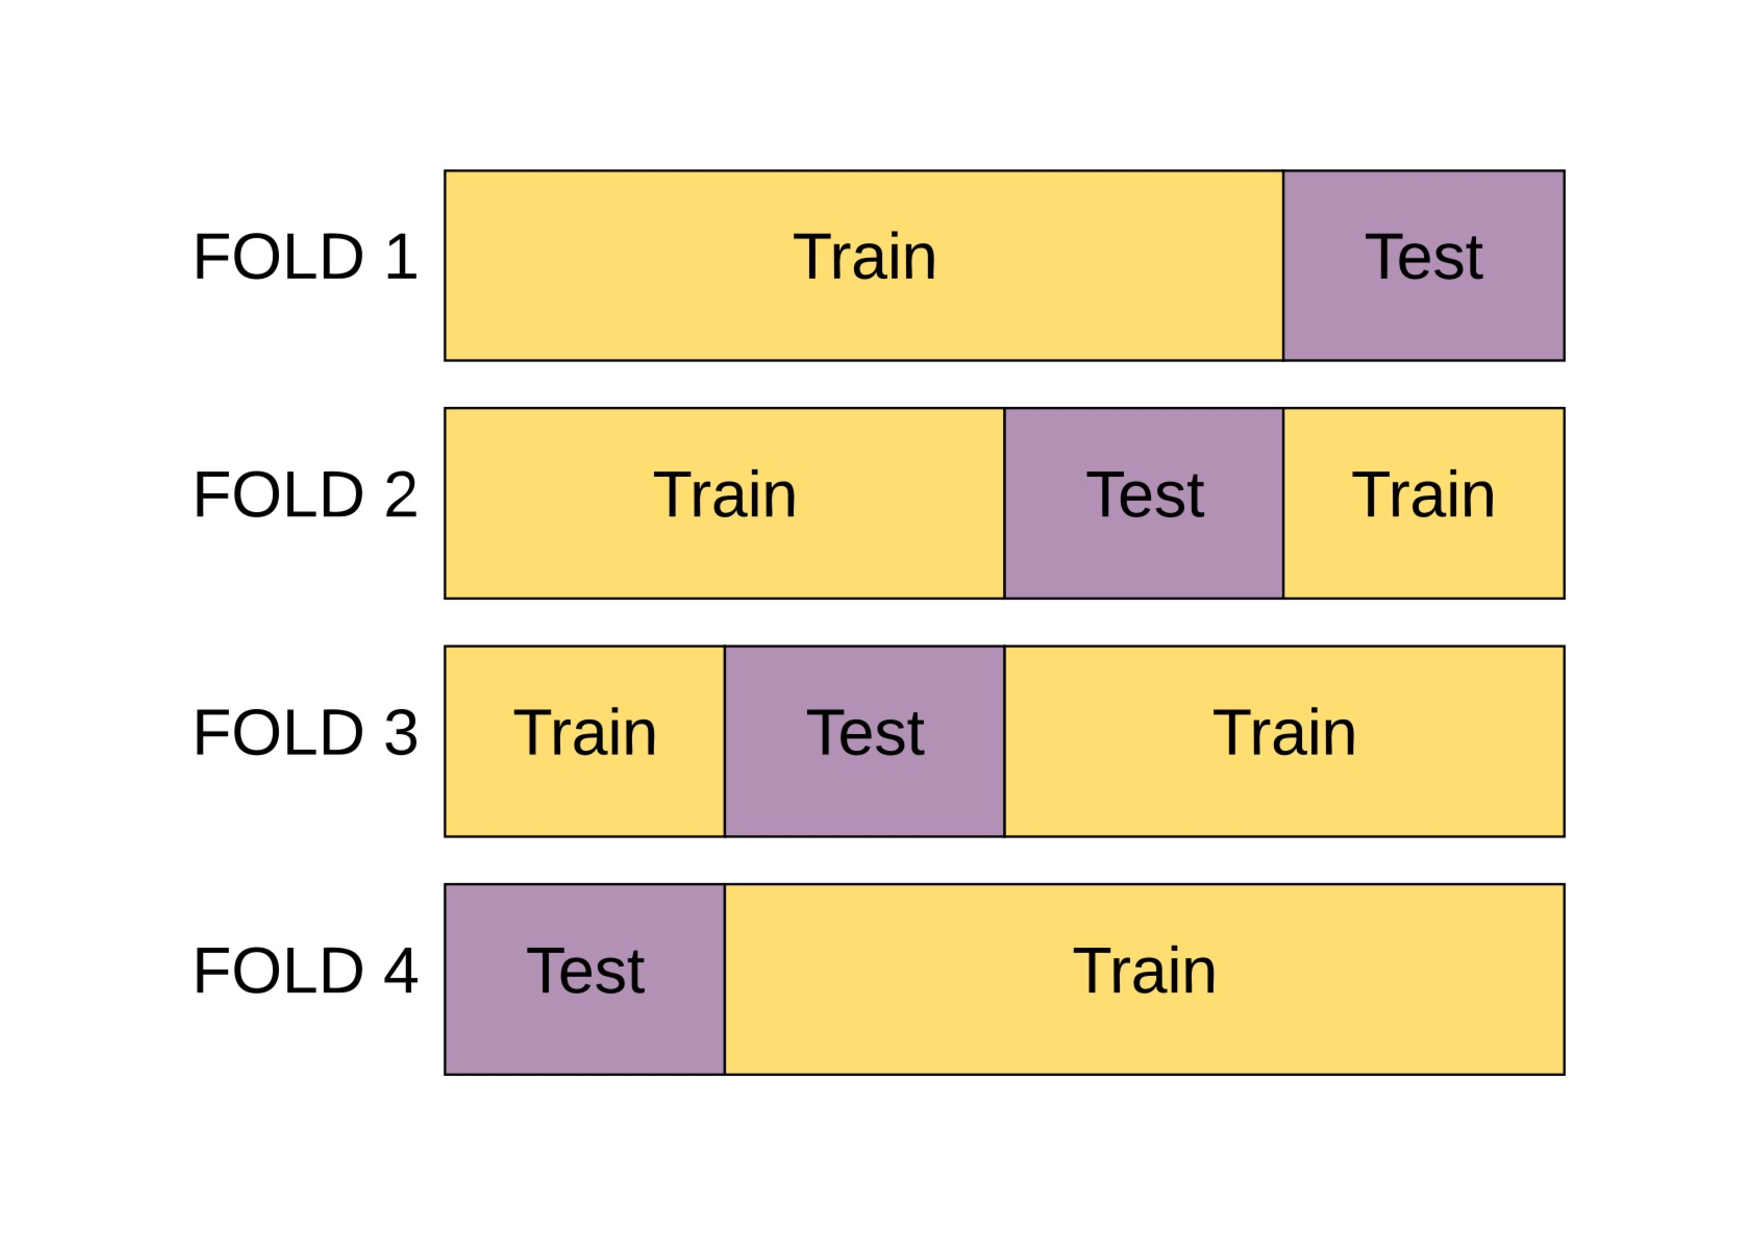
\includegraphics[width = \textwidth]{../assets/bias-variance/diagrams/cross-validation-train-test.pdf}
	\end{frame}

	\begin{frame}{The Validation Set}
	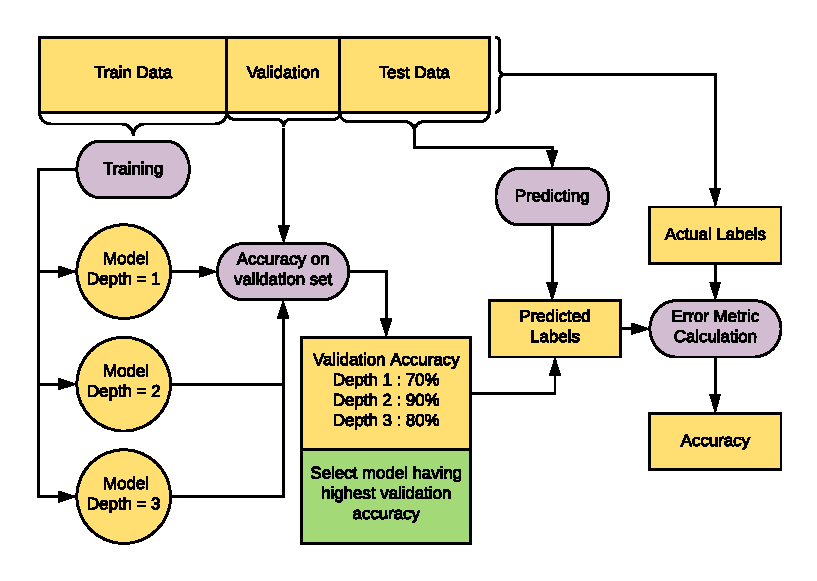
\includegraphics[width = \textwidth]{../assets/bias-variance/diagrams/validation-workflow}
	\end{frame}

	\begin{frame}{Nested Cross Validation}
	Divide your training set into $k$ equal parts.\\
	 Cyclically use 1 part as ``validation set'' and the rest for training.\\
	Here $k = 4$
	\begin{center}
	
\includegraphics[scale=0.7]{../assets/bias-variance/diagrams/cross-validation}
	\end{center}
	\end{frame}

	\begin{frame}{Nested Cross Validation}
	Average out the validation accuracy across all the folds\\
	Use the model with highest validation accuracy\\
	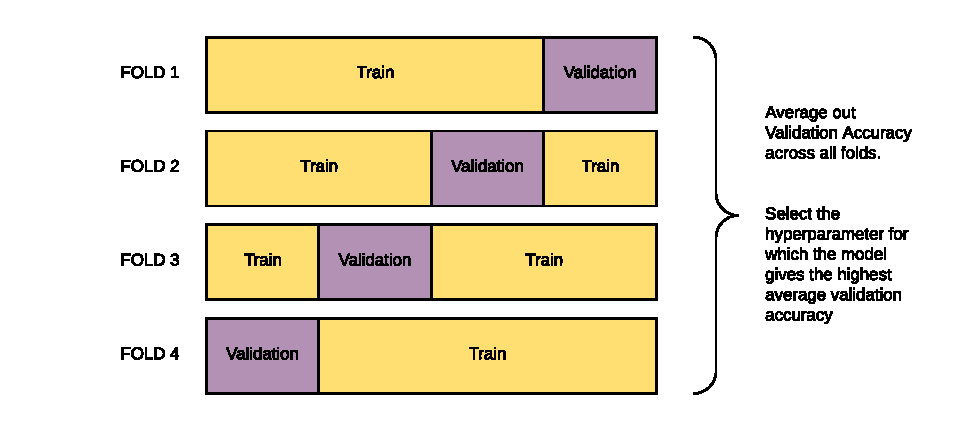
\includegraphics[width = \textwidth]{../assets/bias-variance/diagrams/cross-validation-avg}
	\end{frame}

\section{Practice and Review}

\begin{frame}{Pop Quiz: Bias-Variance Concepts}
\begin{enumerate}
\item What causes high bias in a model? Give an example.
\pause
\item What causes high variance in a model? Give an example.
\pause
\item How does cross-validation help in model selection?
\pause
\item Why can't we directly optimize for test error?
\end{enumerate}
\end{frame}

\begin{frame}{Key Takeaways}
\begin{itemize}[<+->]
\item \textbf{Bias-Variance Decomposition}: Total error = Bias² + Variance + Noise
\item \textbf{High Bias}: Underfitting, model too simple
\item \textbf{High Variance}: Overfitting, model too complex
\item \textbf{Cross-Validation}: Essential for proper model evaluation
\item \textbf{Model Selection}: Choose complexity that balances bias and variance
\item \textbf{No Free Lunch}: Cannot reduce both bias and variance simultaneously
\end{itemize}
\end{frame}

\begin{frame}{Next time: Ensemble Learning}
\begin{itemize}
	\item How to combine various models?
	\item Why to combine multiple models?
	\item How can we reduce bias?
	\item How can we reduce variance?
\end{itemize}
\end{frame}

\end{document}
